\clearpage
\section{Signal models and efficiencies\label{sec:signal}}

\subsection{Introduction}

As described in section~\ref{sec:SUSY}, SUSY is a theory of many particles
and parameters. In order to provide experiments with clear detectable
signatures to search for, simplifed models (SMS) have been derived~\cite{Alwall:2008ag,Alwall:2008va,sms}
which reduce both particles and parameters. In this work, the results are
interpreted in two SMS models:  
\begin{itemize}
\item{T2cc: pair produced stop sparticles each decaying into a charm quark 
and a neutralino}
\item{T2tt; pair produced stop sparticles each decaying into a top quart and a neutralino.}
\end{itemize}
SMS MC samples are generated at leading order with \MADGRAPH~\cite{madgraph} by 
the CMS SUSY MC group and binned in stop mass (mStop) and neutralino mass (mLSP). 
The analysis efficieny is studied in the usual \njet, \nb, \scalht, binning
but due to computational limitations not all categories are used to set 
a limit on a given model. The choice of categories for a model is made by
computing the expected upper limit on the signal cross-section for each
category seperatly using the much quicker asymptotic method~\cite{Cowan:2010js}. 
The categories are ranked by their expected upper limit. Depending on the number of 
mass bins and number of events per bin, two or more categories with the 
higest rank are chosen. The simplified models, along with the event categories 
considered for each, is summarised in Table~\ref{tab:simplified-models}.

\begin{table}[h!]
  \caption{A summary of the simplified models considered for
    interpretation. The event categories considered for each model are
    listed.}  
  \label{tab:simplified-models}
  \setlength{\extrarowheight}{2.5pt}
  \centering
  \begin{tabular}{ llcc }
    \hline
    \hline
    Model             & Production/decay mode & (\njet,\nb) event categories considered        \\ 
    \hline
    \texttt{T2cc}     & \Ttwocc               & (2--3,0), ($\geq 4$,0), ($\geq 4$,1) \\ % (2--3,1), 
    \texttt{T2tt}     & \Ttwott               & ($\geq 4$,1), ($\geq 4$,2) \\
    \hline
    \hline
  \end{tabular}
\end{table}

\subsection{Efficiency times acceptance\label{sec:t2cc-eff}}

The signal efficiency times acceptance is measured in the same binning
as the analysis binning (\njet,\nb,\scalht). To reduce the number of
figures in this section to a manageable level, only the total efficiency for
the relevant event categories and inclusive selection on \scalht ($>375\gev$) 
is shown. Figures~\ref{fig:sms-eff-t2cc} and~\ref{fig:sms-eff-t2tt} show the
expected signal efficiency times acceptance for the hadronic selection
the \verb!T2cc! and \verb!T2tt! interpretations for categories of interest.

\begin{figure}[h!]
  \begin{center}
    \subfigure[Hadronic Selection Efficiency, (2--3,0)]{
      \includegraphics[width=0.4\textwidth,page=6]{figures/sms/t2cc/v1/T2cc_eff}
    } 
    \subfigure[Hadronic Selection Efficiency, (2--3,1)]{
      \includegraphics[width=0.4\textwidth,page=7]{figures/sms/t2cc/v1/T2cc_eff}
    } 
    \subfigure[Hadronic Selection Efficiency, ($\geq 4$,0)]{
      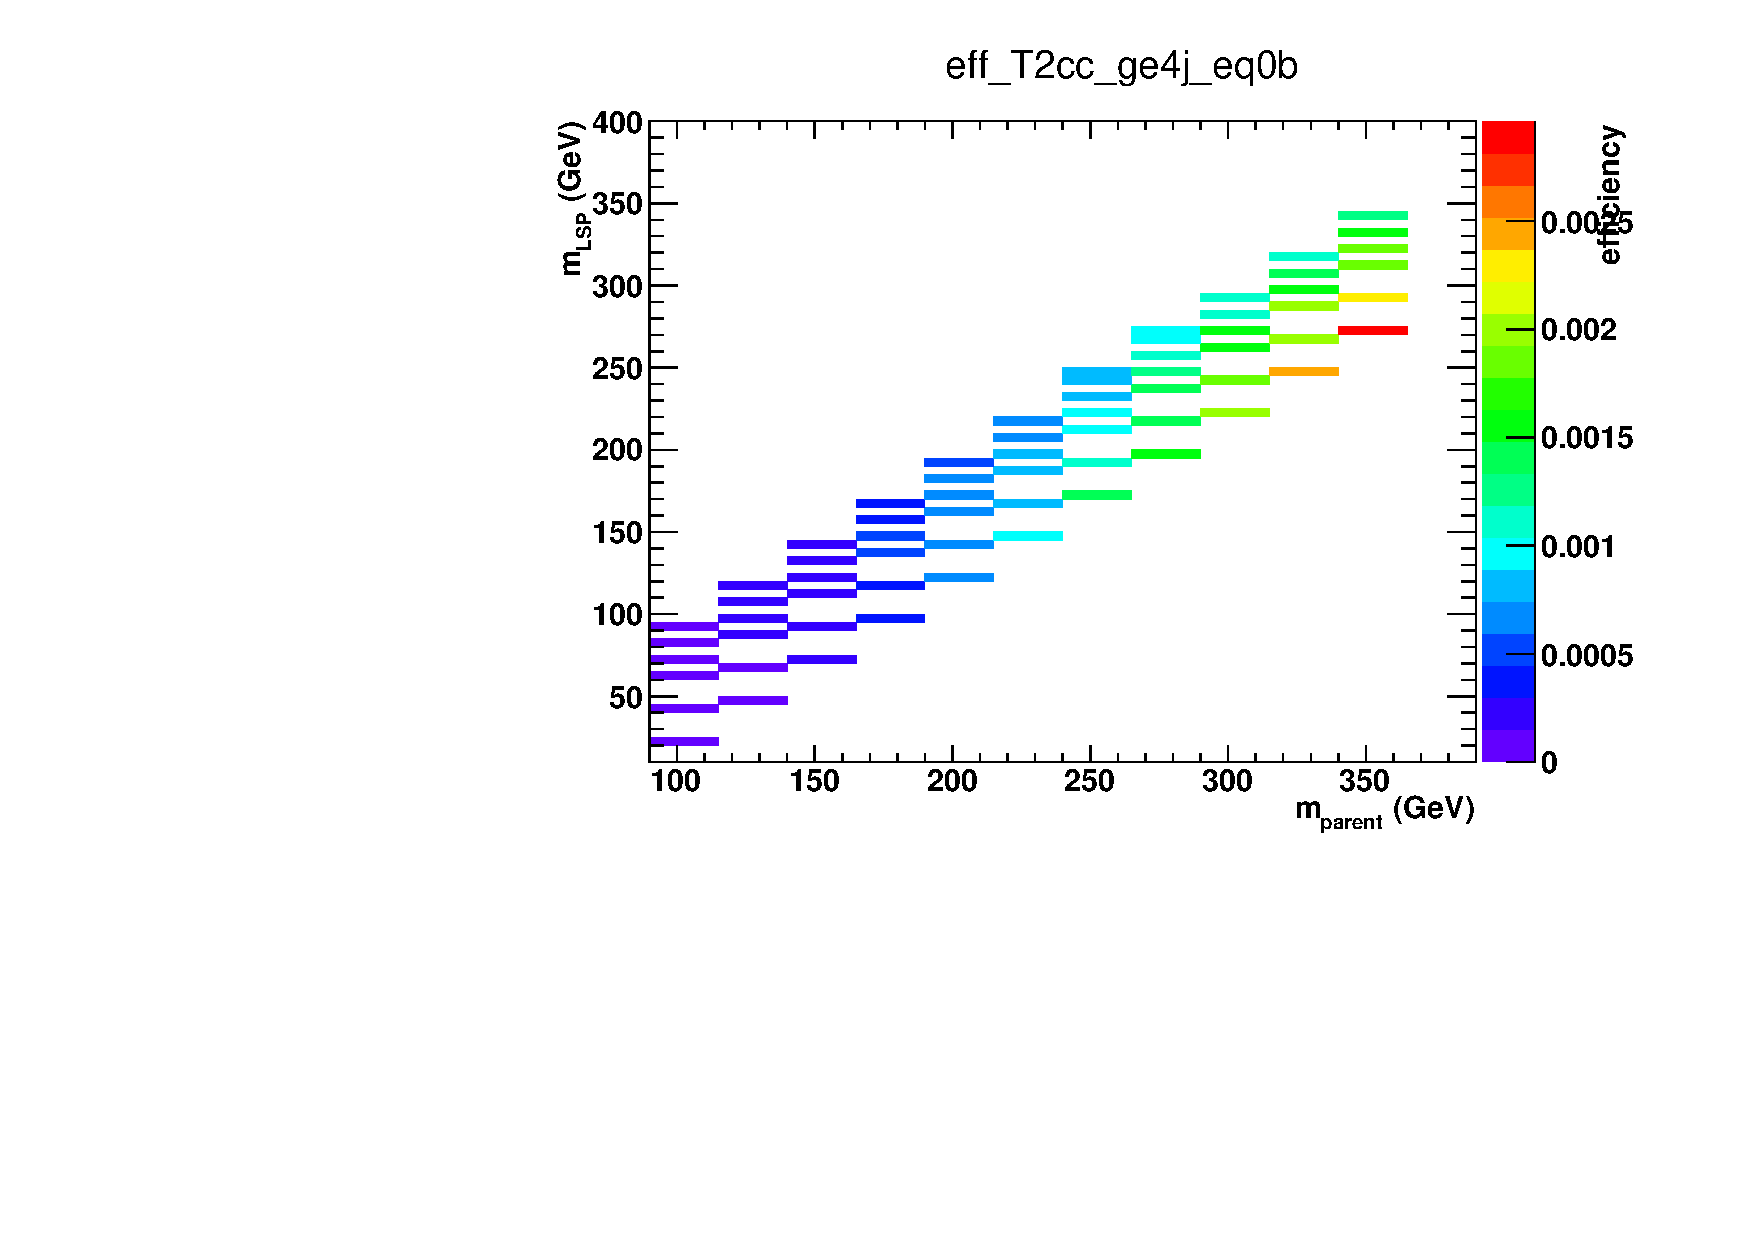
\includegraphics[width=0.4\textwidth,page=1]{figures/sms/t2cc/v1/T2cc_eff}
    } 
    \subfigure[Hadronic Selection Efficiency, ($\geq 4$,1)]{
      \includegraphics[width=0.4\textwidth,page=2]{figures/sms/t2cc/v1/T2cc_eff}
    } 
    \caption{Hadronic selection efficiency times acceptance for \texttt{T2cc}
      for the relevant event categories defined by \njet and \nb.
      Note the different z-axis scales.}
    \label{fig:sms-eff-t2cc}
  \end{center}
\end{figure}

\begin{figure}[!h]
  \begin{center}
    \subfigure[Hadronic Selection Efficiency, ($\geq 4$,1)]{
      \includegraphics[width=0.4\textwidth,page=2]{figures/sms/t2tt/v1/T2tt_eff}
    } 
    \subfigure[Hadronic Selection Efficiency, ($\geq 4$,2)]{
      \includegraphics[width=0.4\textwidth,page=3]{figures/sms/t2tt/v1/T2tt_eff}
    } \\
    \caption{Hadronic selection efficiency times acceptance for the \texttt{T2tt}
      for the relevant event categories defined by \njet and \nb.
       Note the different z-axis scales.}
    \label{fig:sms-eff-t2tt}
  \end{center}
\end{figure}

In \verb!T2cc!, the decay quarks become virtually undetectable as 
the nearly degenerate parent and daugther masses leave litte energy for the decay 
products. Therfore any analysis interpreting in the \verb!T2cc! model 
relies on hard-\Pt jets from initial state radiation for acceptance. The 
efficiency times acceptance is below the percent level where The largest 
efficiencies for the smallest mass splittings, $\Delta M = \sim10\gev$, 
are obtained with the (2--3,0) category, while for larger mass splittings 
the (2--3,1), ($\geq 4$,0), and ($\geq 4$,1) categories contribute 
due to the reduced backgrounds in these categories. In \verb!T2tt! the largest
efficiencies are obtained in largest mass splittings in both categories of interest. 
In both models, the signal efficiency in the \mj control sample is negligible 
with respect to the signal region. 

\clearpage
\section{Systematic uncertainties on signal efficiency times 
  acceptance\label{sec:sms-syst}}

\subsection{Introduction} 

To gain statistical power, The systematic uncertainty in the signal 
acceptance times efficiency is determined per mass point per event 
category (\njet,\nb), but inclusively in \scalht . This section details the methods 
used to determine the magnitude of the systematic uncertainties to be applied. 
Four sources of uncertainty are measured: the jet energy scale,
the parton distribution functions, initial state radiation and b-tag scale
factors. Three other uncertainties are quoted: the uncertainty in the luminosity (2.6\%) and
trigger (5\%) measurments and the ``dead ECAL'' filter (3 \%) used in the candidate signal
event selection. Each contribution is considered to be independent 
and all contributions are summed in quadrature to obtain a total 
systematic uncertainty per mass point per category.

The following sub-sections provide an overview of the various sources of
uncertainty, before details on specific models are provided. 

\subsection{PDF uncertainties\label{sec:pdf-sets}}

The simulated signal events were produced with the \verb!CTEQ6L1! PDF
set by default.  As recommended by PDF4LHC~\cite{pdf4lhc}, the uncertainty
in signal efficiency due to knowledge of the PDFs is obtained by comparing 
the signal efficiency with that obtained with three newer alternative PDF 
sets: \verb!CT10!, \verb!NNPDF2.1!, and \verb!MSTW2008!. Using the envelope
formula in the reference, a single efficiency is calculated from the three alternate
PDF sets. 

Figures~\ref{fig:sms-pdf-t2cc} and~\ref{fig:sms-pdf-t2tt} 
(Appendix~\ref{app:signal}) show the relative difference of the signal 
efficiency times acceptance for the central value of the envelope calculation 
and the nominal PDF (\verb!CTEQ6L1!) set used to produce the signal 
samples. The relative difference is taken as a symmetric systematic 
uncertainty, which varies in absolute terms within the range 0--10\% in 
in both models depending on the category of interest.

\subsection{Jet energy scale\label{sec:sms-syst-jes}}

Figures~\ref{fig:sms-jes-t2cc} and ~\ref{fig:sms-jes-t2tt} 
(Appendix ~\ref{app:signal}) show the relative change in the 
signal efficiency times acceptance for the relevant categories for 
the \verb!T2cc! and \verb!T2tt! interpretations when varying the energy 
of all jets in an event up or down according to a \pt- and $\eta$-dependent 
jet energy scale uncertainty, as recommended by the JetMET POG. 
In \verb!T2cc!, larger variations are observed for the higher 
jet multiplicity category, as as the jets are softer for the same 
requirement on \scalht. Also, the variations may increase with 
increasing mass splitting as additional (soft) jets from the decay 
become hard enough to move within acceptance. The variations in both 
signal models range between $\sim5\%$ and $\sim15\%$ for the low 
and high jet multiplicity, and are largely independent of parent 
and daughter sparticle mass. 

\subsection{Initial state radiation\label{sec:sms-syst-isr}}

Signal samples produced with \MADGRAPH exhibit discripencies that 
have been attributed to the mismodelling of initial state radiation.
These discripencies are corrected as recommended by the SUSY 
PAG~\cite{susy-isrrw}. As per prescripton, events are reweighted
according to the vectorial sum of the momenta of the pair-produced
sparticles. The sparticle-system \Pt dependent weights are summarized in  
Table~\ref{tab:sms-syst-isr-factors}.   In addition to the central weight, 
further variations about the central weight according to the uncertainty 
in the weight is applied in order to determine the systematic uncertainty
associated with the correction. The resulting systematic uncertainties 
are largest near the diagonal where selected events contain significant 
amounts of boost due to the presence of initial state radiation. 

Figure~\ref{fig:sms-isr-t2cc} and~\ref{fig:sms-isr-t2tt} 
(Appendix ~\ref{app:signal}) shows the relative change in the signal 
efficiency times acceptance for the relevant categories for the 
\verb!T2cc! and \verb!T2tt! interpretation when varying up and down
the sparticle system \Pt-dependent corrections by their
uncertainties. The largest variations, up to $\sim25\%$ are observed
for the smallest mass splittings, when the reliance on ISR jets for
acceptance is largest. 

\begin{table}[!h]
  \caption{Sparticle system \Pt dependent corrections and systematic
    weight variations.} 
  \label{tab:sms-syst-isr-factors}
  \centering
  \footnotesize
  \begin{tabular}{ lcc }
    \hline
    Sparticle system \Pt (GeV) & Central Weight & Systematic Variation \\
    \hline
    $0 < \Pt < 120$            & 1.00           & $\pm$ 0.0            \\
    $120 < \Pt < 150$          & 0.95           & $\pm$ 0.05           \\
    $150 < \Pt < 250$          & 0.90           & $\pm$ 0.10           \\
    $\Pt > 250$                & 0.80           & $\pm$ 0.20           \\
    \hline
    \hline
  \end{tabular}
\end{table}

\subsection{b-tag scale factor corrections\label{sec:sms-syst-btag}}

The uncertainty on the btag scale factors described in section [REF]
is calculated by varying the scale factors up and down by their
uncertainty as described in Ref.~\cite{btagpogtwiki}.

Figure~\ref{fig:sms-btag-t2cc} and~\ref{fig:sms-btag-t2tt} (Appendix ~\ref{app:signal})
show the relative change in the signal efficiency times acceptance for 
the relevant categories for the \verb!T2cc! and \verb!T2tt! interpretations
when varying up and down the scale-factor corrections by their uncertainties. 
The variations  are anti-correlated for the two \nb categories used by this
interpretation and are generally small, at the level of 1--5\%, with
respect to other contributions. 

\subsection{Total systematic uncertainties\label{sec:total-sms-unc}}

A few mass bins exhibit large uncertainties compaired to neighboring 
mass bins.  This effect atributed to low statitics when calculating the signal
efficiency times acceptance in that bin. In order to decouple systematic
and statistical uncertainties, these values have been replaced with appropriate 
values (determined by neighboring bins) in the calculation of the
total uncertainty. Hence, figures ~\ref{fig:sms-total-t2cc} and
~\ref{fig:sms-total-t2cc}, rerpresenting the total
systematic uncertainty in the \verb!T2cc! and \verb!T2tt! interpretations
for relevant categories are devoid of such fluctations.

\begin{figure}[h!]
  \begin{center}
    \subfigure[\njetlow, $\nb = 0$.]{
     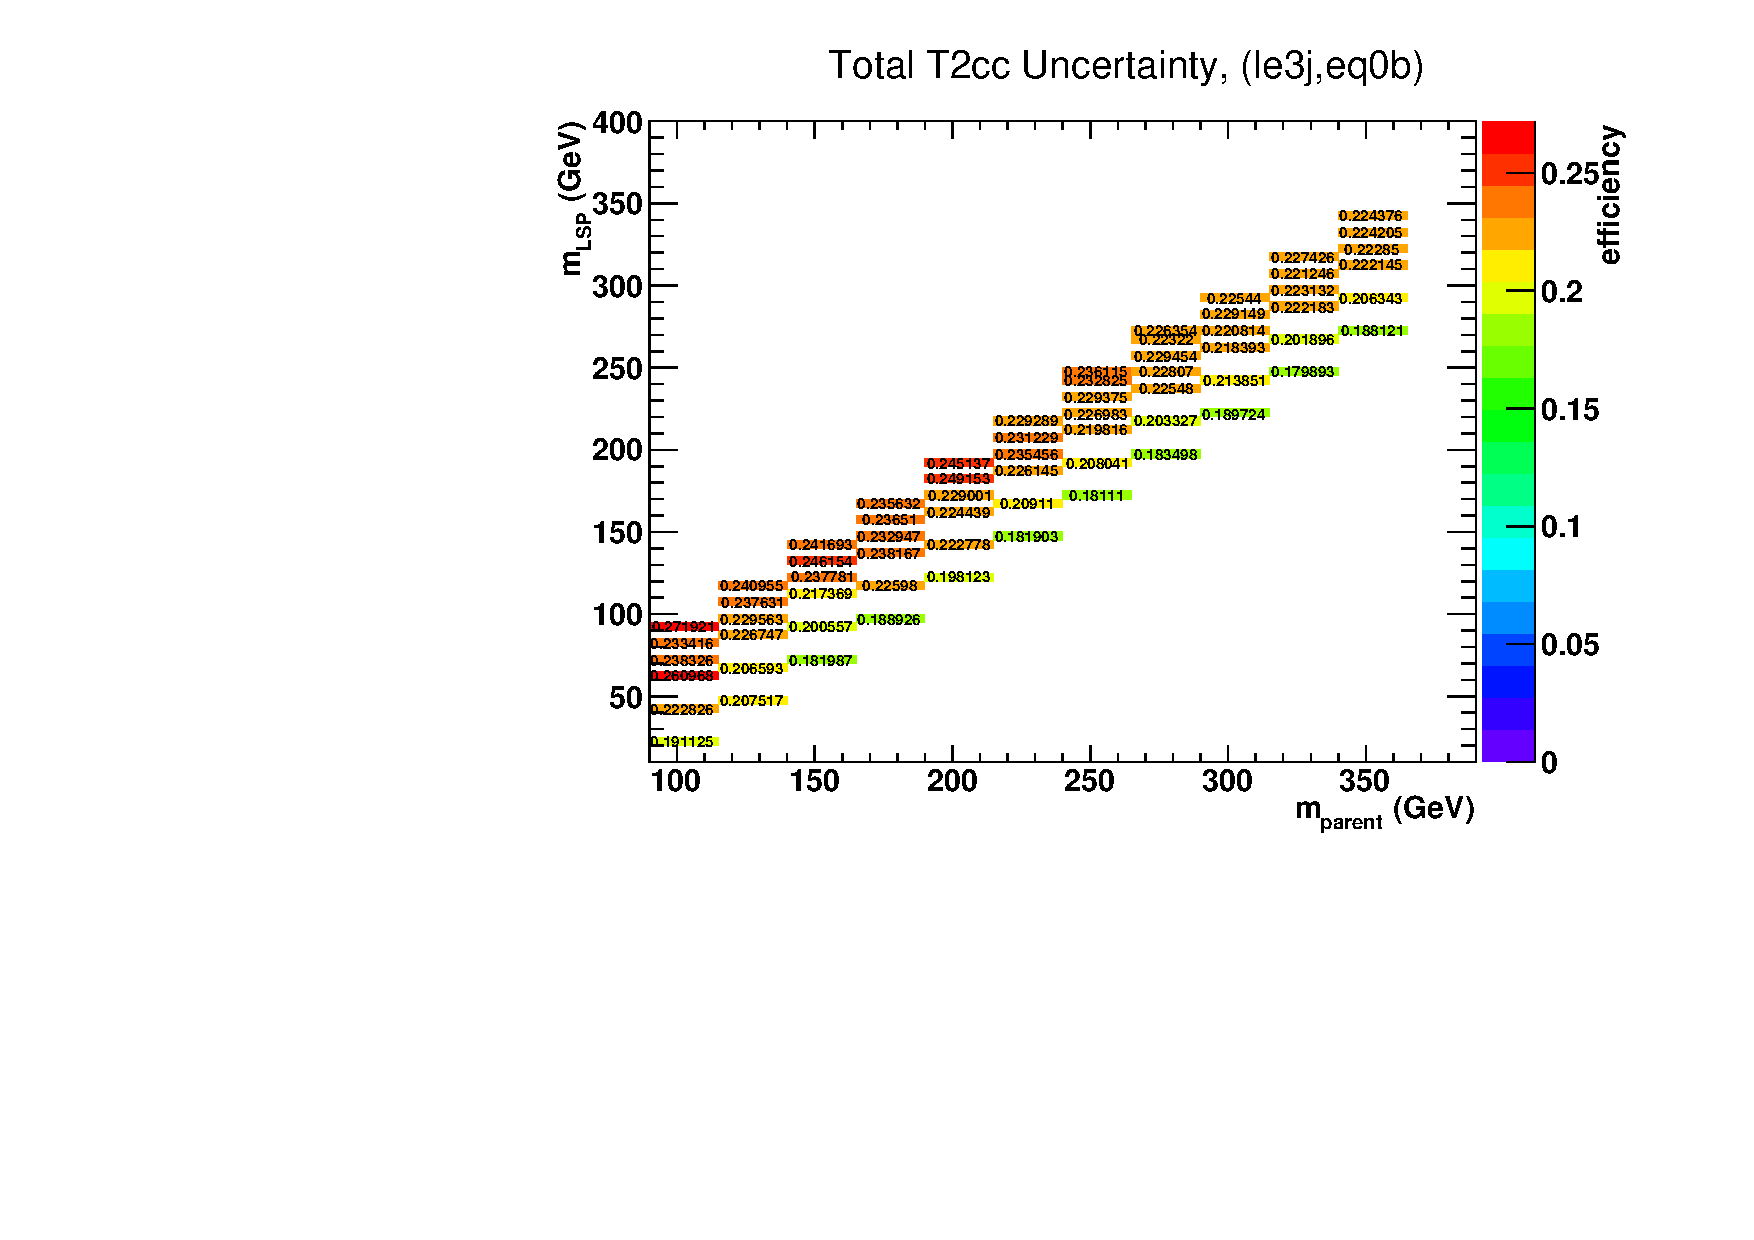
\includegraphics[width=0.48\textwidth,page=1]{figures/sms/t2cc/v1/t2cc_pfJet_totalUnc.pdf}
    }                                                                  
    \subfigure[\njetlow, $\nb = 1$.]{                                  
     \includegraphics[width=0.48\textwidth,page=2]{figures/sms/t2cc/v1/t2cc_pfJet_totalUnc.pdf}
    }\\                                                                
    \subfigure[\njethigh, $\nb = 0$.]{                                 
      \includegraphics[width=0.48\textwidth,page=5]{figures/sms/t2cc/v1/t2cc_pfJet_totalUnc.pdf}
    }                                                                  
    \subfigure[\njethigh, $\nb = 1$.]{                                 
      \includegraphics[width=0.48\textwidth,page=6]{figures/sms/t2cc/v1/t2cc_pfJet_totalUnc.pdf}
    }\\
    \caption{\label{fig:sms-total-t2cc}The total systematic
      uncertainty in the signal efficiency times acceptance for all
      relevant event categories for the \texttt{T2cc} intepretation.}
  \end{center}
\end{figure}


\begin{figure}[h!]
  \begin{center}
    \subfigure[\njethigh, $\nb = 1$.]{
     \includegraphics[width=0.48\textwidth,page=2]{figures/sms/t2tt/v1/t2tt_pfJet_totalUnc.pdf}
    }
    \subfigure[\njethigh, $\nb = 2$.]{
     \includegraphics[width=0.48\textwidth,page=3]{figures/sms/t2tt/v1/t2tt_pfJet_totalUnc.pdf}
    }\\       
    \caption{\label{fig:sms-total-t2tt}The total systematic
      uncertainty in the signal efficiency times acceptance for all
      relevant event categories for the \texttt{T2tt} intepretation.}
  \end{center}
\end{figure}

Table~\ref{tab:sms-syst-t2cc} presents a {\it representative} range of
values for the contribution to the total systematic uncertainty in the
signal efficiency times acceptance for each relevant event
category. An uncertainty of 2.6\% in the integrated luminosity is also
considered. An uncertainty of 5\% from the trigger uncertainty measurment
Figure~\ref{fig:sms-total-t2cc} shows the total systematic uncertainty 
in the \verb!T2cc! mass plane for the relevant categories.

\begin{table}[h!]
  \caption{Representative ranges for each contribution to the total
    systematic uncertainty in the signal efficiency times acceptance
    for each relevant event category for the \texttt{T2cc}
    interpretation.
    \label{tab:sms-syst-t2cc}
  }   
  \centering
  \begin{tabular}{ lcccccccc }
    \hline
    \hline
    Category   & \multicolumn{2}{c}{(2--3,0)} & \multicolumn{2}{c}{($\geq 4$,0)} & \multicolumn{2}{c}{($\geq 4$,1)} & \multicolumn{2}{c}{($\geq 2$,$\geq 0$)} \\
    Range      & Min.   & Max.                & Min.   & Max.                    & Min. & Max.                      & Min.  & Max.        \\
    \hline
    PDF        & 0.00   & 0.05                & 0.00   & 0.05                    & 0.00 & 0.10                      &         \\
    JES        & 0.00   & 0.10                & 0.00   & 0.10                    & 0.00 & 0.15 	                    &             \\
    ISR        & 0.15   & 0.25                & 0.10   & 0.15                    & 0.15 & 0.30 	                    &             \\
    b-tag SF   & 0.00   & 0.08                & 0.00   & 0.10                    & 0.00 & 0.15 	                    &             \\
    Luminosity &        &                     &        &                         &      &      	                    & 0.026 & 0.026        \\
    Trigger    &        &                     &        &                         &      &                           & 0.05 & 0.05        \\
    Dead Ecal  &        &                     &        &                         &      &      	                    & 0.03 & 0.03        \\
    \hline
    Total syst & 0.18   & 0.25                & 0.19   & 0.30                    & 0.20 & 0.38                      &      &             \\
    \hline
    \hline
  \end{tabular}
\end{table}


\begin{table}[h!]
  \caption{Representative ranges for each contribution to the total
    systematic uncertainty in the signal efficiency times acceptance
    for each relevant event category for the \texttt{T2tt}
    interpretation.
    \label{tab:sms-syst-t2cc}
  }   
  \centering
  \begin{tabular}{ lcccccccc }
    \hline
    \hline
    Category   & \multicolumn{2}{c}{($\geq 4$,1)} & \multicolumn{2}{c}{($\geq 4$,2)}  & \multicolumn{2}{c}{($\geq 2$,$\geq 0$)} \\
    Range      & Min.   & Max.                & Min.   & Max.                     & Min.  & Max.        \\
    \hline
    PDF        & 0.00   & 0.10                & 0.00   & 0.10                     &         \\
    JES        & 0.00   & 0.10                & 0.00   & 0.05                     &             \\
    ISR        & 0.00   & 0.20                & 0.00   & 0.22                     &             \\
    b-tag SF   & 0.00   & 0.05                & 0.00   & 0.10                     &             \\
    Luminosity &        &                     &        &                          & 0.026 & 0.026        \\
    Trigger    &        &                     &        &                          & 0.05 & 0.05        \\
    Dead Ecal  &        &                     &        &                          & 0.03 & 0.03        \\
    \hline
    Total syst & 0.05   & 0.25                & 0.05   & 0.30                     &      &             \\
    \hline
    \hline
  \end{tabular}
\end{table}

